\section{Hardware}
\subsection{Sensor Node}
The sensor node is constituted by the panstamp, an accelerometer and a voltage divisor circuit.

\subsubsection{Accelerometer}
The ADXL335 is a small low power 3-axis accelerometer that measures acceleration with a range of at least +/- 3g; in other words, +/- 3g is the maximum amplitude that this accelerometer can detect before distorting or clipping its output signal. 1g is the acceleration due to the earth's gravity (9.8 m/sec2).

According to the ADXL335 datasheet (add reference), the capacitors Cx, Cy and Cz connected to the accelerometer pins Xout, Yout and Zout determine the accelerometer's bandwidth. With these capacitors, a low pass-filter for anti-aliasing and noise reduction is implemented. In the board GY-61 (see Figure~\ref{fig:accelerometer}), Cx, Cy and Cz have a capacitance of 0.1uF that yields a bandwidth of 50 Hz (add reference). 	

To minimize aliasing, the accelerometer's analog bandwidth must be no more than half the analog-to-digital sampling frequency. Therefore, the panstamp was programmed to sample the accelerometer's signal at a frequency of 200z (see Driver section), thus the analog-to-digital sampling frequency is 4 times the accelerometer's analog bandwidth. 

\begin{figure}[h!] 
 \centering
 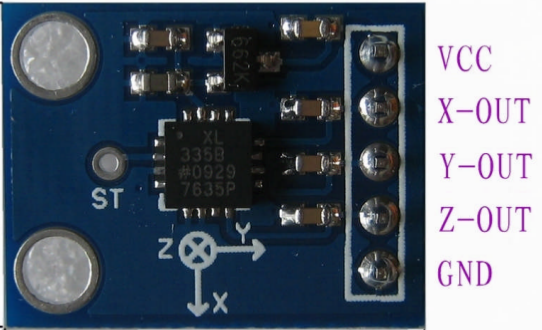
\includegraphics[width= 0.35\textwidth, clip=true,keepaspectratio=true]
 {./pic/accelerometer.png}
 \caption{ADXL335 accelerometer in board GY-61}
 \label{fig:accelerometer}
\end{figure}  
    
  
\subsubsection{Voltage monitoring circuit}
To detect when the Li-Po battery has low voltage, a voltage monitoring circuit was implemented with the Panstamp's analog comparator module (add reference to the data-sheet here) and a voltage divisor circuit (see Figure~\ref{fig:voltage-monitor}). According to the ATMEGA 328 data-sheet (add reference), the Analog Comparator compares the input values on the positive pin AIN0 and negative pin AIN1. 

In our implementation, the Analog Comparator triggers an interruption in the sensor node when the voltage on the pin AIN0 decreases below the voltage in pin AIN1. With the configuration shown in Figure~\ref{fig:voltage-monitor}, the voltage in AIN1 is always 2.4 V. When the Li-po battery voltage falls below 9.5 Volts, the voltage in AIN0 (which is the same voltage in resistor R2) is less than the voltage in AIN1 and the Analog Compator activates as a result an interruption.

To minimize power dissipation in the voltage monitoring circuit, the possible maximum current in brach R1-R2 and in branch R3-R4 was fixed to 0.1mA. With this value and the maximum voltage given by the Li-po battery (12.5 V) the values of R1, R2, R3 and R4 were calculated.  

\begin{figure}[h!] 
 \centering
 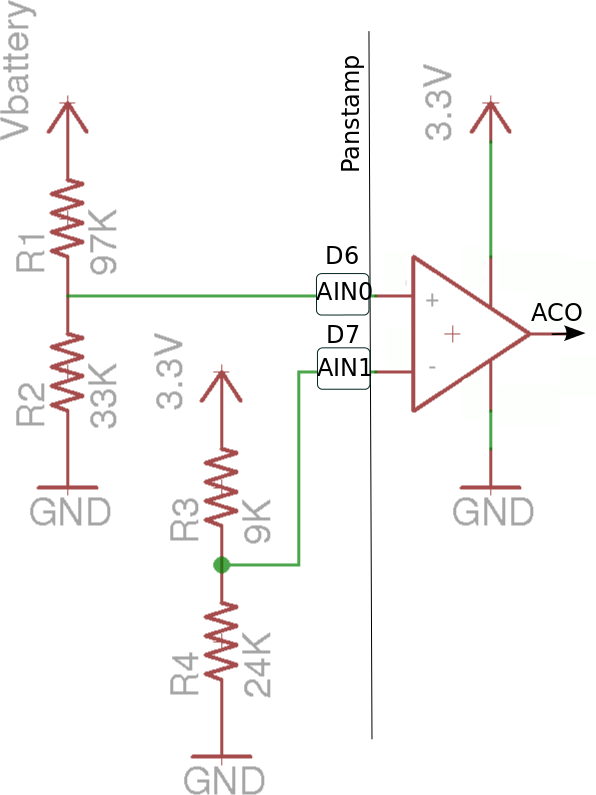
\includegraphics[width= 0.35\textwidth, clip=true,keepaspectratio=true]{./graph/voltage_comparator_circuit.png}
 \caption{Voltage monitoring circuit}
 \label{fig:voltage-monitor}
\end{figure}

\subsection{Actuator Node}
The actuator node is constituted by a panstamp and a led strand, whose length varies among the different modules. 
\subsubsection{Led strand}
In the led strand, each pixel contains a small microchip called LPD6803 and both led and chip are encapsulated within a silicone enclosure . Thanks to this microchip, each pixel in the strand can be controlled individually. It is recommended to use a supply voltage of 5 volts for the led strand (See LPD6803 datasheet). As shown in Figure~\ref{fig:led-strand}, the led strand has 4 cables: the red and white ones are for the power supply (red is positive and white has to be connected to ground), the blue one is the data cable and finally the green one is the clock cable. In our system, blue is connected to the panstamp's digital pin 5 and the green cable is connected to the panstamp's digital pin 3. 

\begin{figure}[h!] 
 \centering
 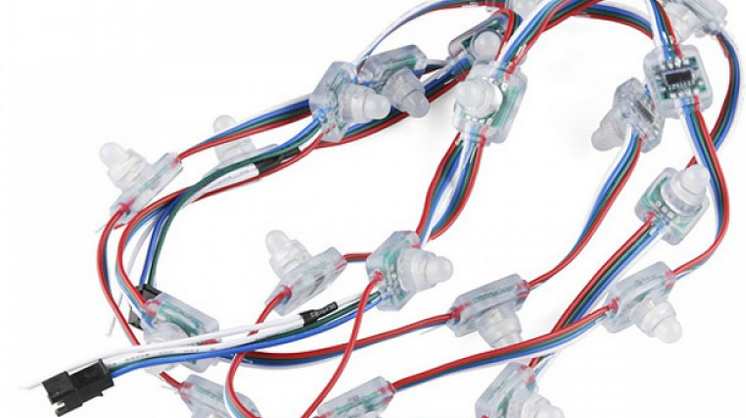
\includegraphics[width= 0.35\textwidth, clip=true,keepaspectratio=true]{./pic/led-strand-all.jpeg}
 \caption{Led strand}
 \label{fig:led-strand}
\end{figure}

\subsection{Server Node}
The sensor node is constituted by a panstamp and a panStick (See Figure~\ref{fig:panstick}).
PanStick is a USB mother board that enables both the programming of panStamps and the communication between a panstamp and a computer via USB.

\begin{figure}[h!] 
 \centering
 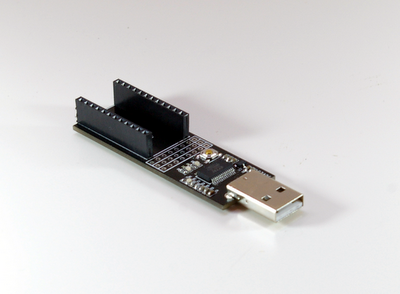
\includegraphics[width= 0.35\textwidth, clip=true,keepaspectratio=true]{./pic/panStick_01.png}
 \caption{Panstick}
 \label{fig:panstick}
\end{figure}

Additionally, the panStick includes a reset button that lets restart an application without having to unplug the board.